%!TEX root = ../dokumentation.tex

\section{Gestaltungslösungen}


\subsection{Prototyping}

Hartmann Seite 442

\subsection{Paperbased Prototyping}

Testen und Modifizieren des neuen Systems in Partnerschaft mit den Benutzern, indem papierbasierte „mock-ups“ des Benutzerinterfaces geschaffen werden. Wirkliche Arbeitsaufgaben mit „Papier- System“ bearbeiten lasseen und nicht nur „reviewen“ sammeln von Einschätzungen

Sicherstellen eines verlässlichen Weges um mit Benutzern über das zu schaffende System zu sprechen. Verifizieren des Entwurfs bevor der codiert wird. Vertiefen der Anforderungen an das System. Frühes Testen von Benutzer- Interface Ideen und Produktkonzeptionen

\subsection{Evaluation}

empirischer Ansatz
Vertreter der Stakeholder ,analytisch nicht möglich, da keine MCI Experten
Hartmann Seite 
Techniken
Think aloud (formativ) während, dient zur Entdeckung, mit benutzerbeteiligung, qualitativ\\
testperson testet system und spricht gedanken laut aus + protokoll
tester, moderator
user testing\\
test mit probanden
problem rahmenbedingungen beeinflussen
observation\\
interpretation des Analysten
survey\\
schwierig da psychologisch
interview\\
cognitive walkthrough\\
	gedankliches Nachverfolgen der Aufgabenerledigung, erlernbarkeit, gebrauchstauglichkeit
expert review\\

Auswahl nach Zielsetzung, Ressourcen, , domänenspezifischer Kontext\\
Zeitpunkt
formative vor oder während vs summative E abschließend\\
hinsichtlich erhobener Daten
qualitative sprachliche Basis vs quantitative E auf Zahlenbasis\\
wissenschaftstheoretische ausrichtung
induktive bottom Einzelbeobachtungen verallgemeinern up vs dediktive E vom allgemeinen zum konkreten top down\\

Auswahl nach Zeitpunkt im EP, Grad der Benutzerbeteiligungm Aufwand, Untersuchungsfokus

Interaktionsphase\\
Durchführungsphase\\
Abschlussphase\\
high fidelty prototype
passiver Prototyp
working prototyp 

Abb. \ref{fig:evaluation11}
\begin{figure}[H]
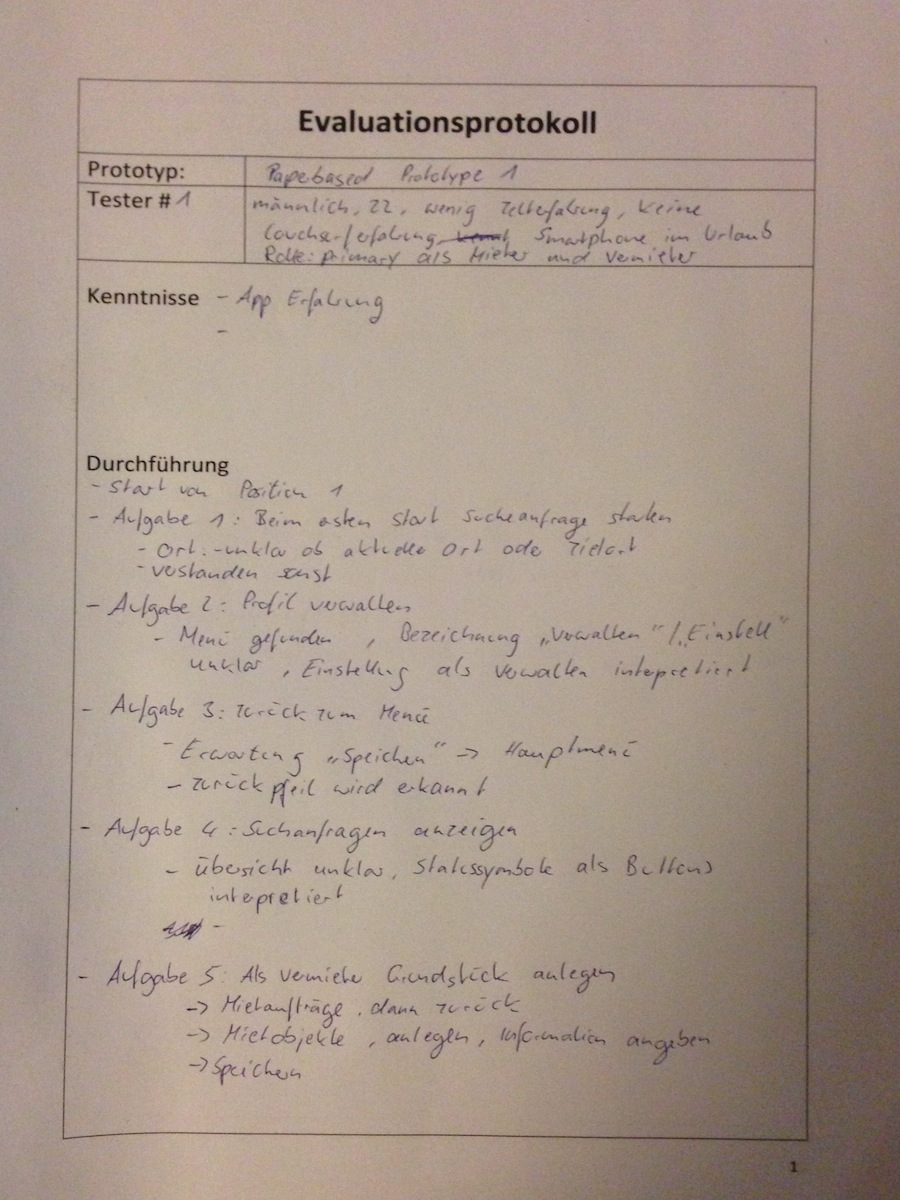
\includegraphics[width=1\textwidth]{./images/evaluation/eva11.JPG}
\caption{Evaluationsprotokoll 1.1}
\label{fig:evaluation11}
\end{figure}

Abb. \ref{fig:evaluation12}
\begin{figure}[H]
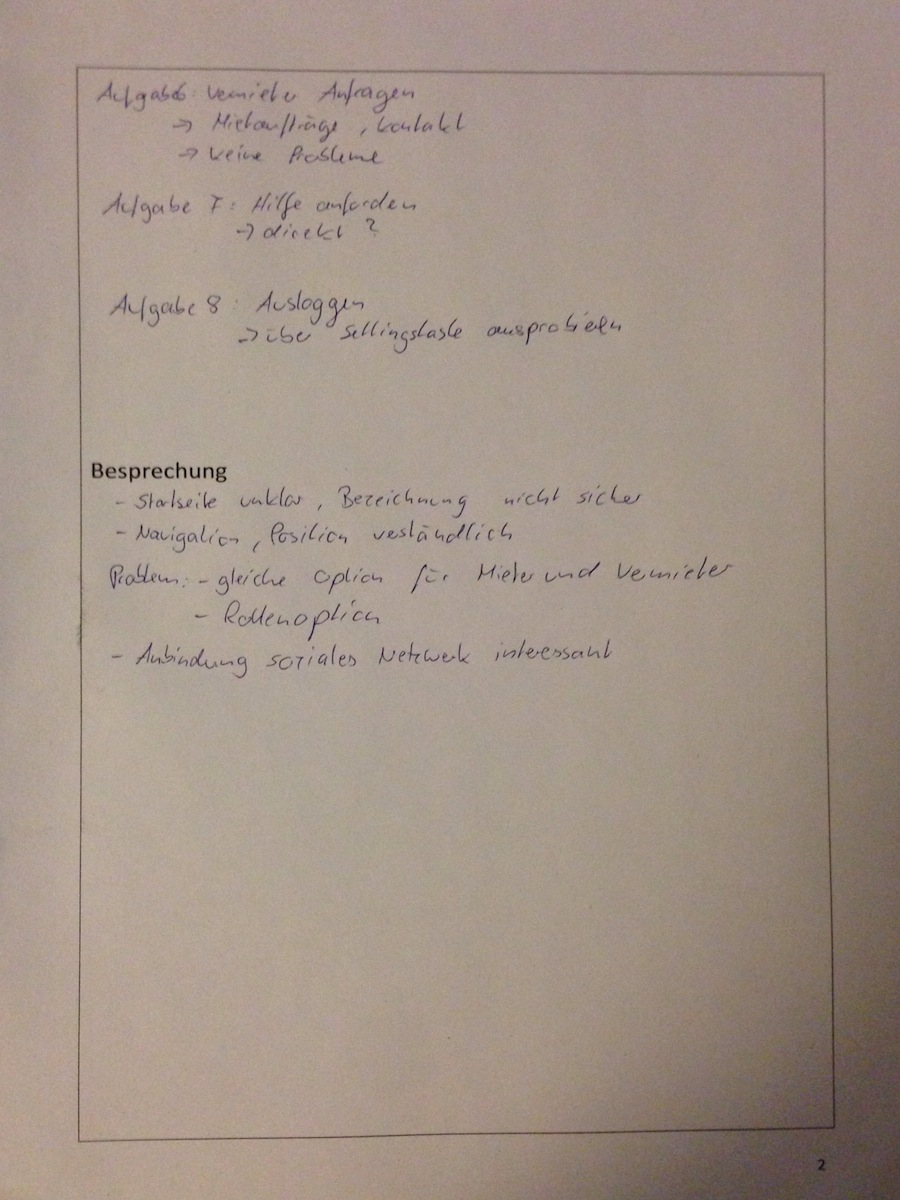
\includegraphics[width=1\textwidth]{./images/evaluation/eva12.JPG}
\caption{Evaluationsprotokoll 1.2}
\label{fig:evaluation12}
\end{figure}

Abb. \ref{fig:evaluation21}
\begin{figure}[H]
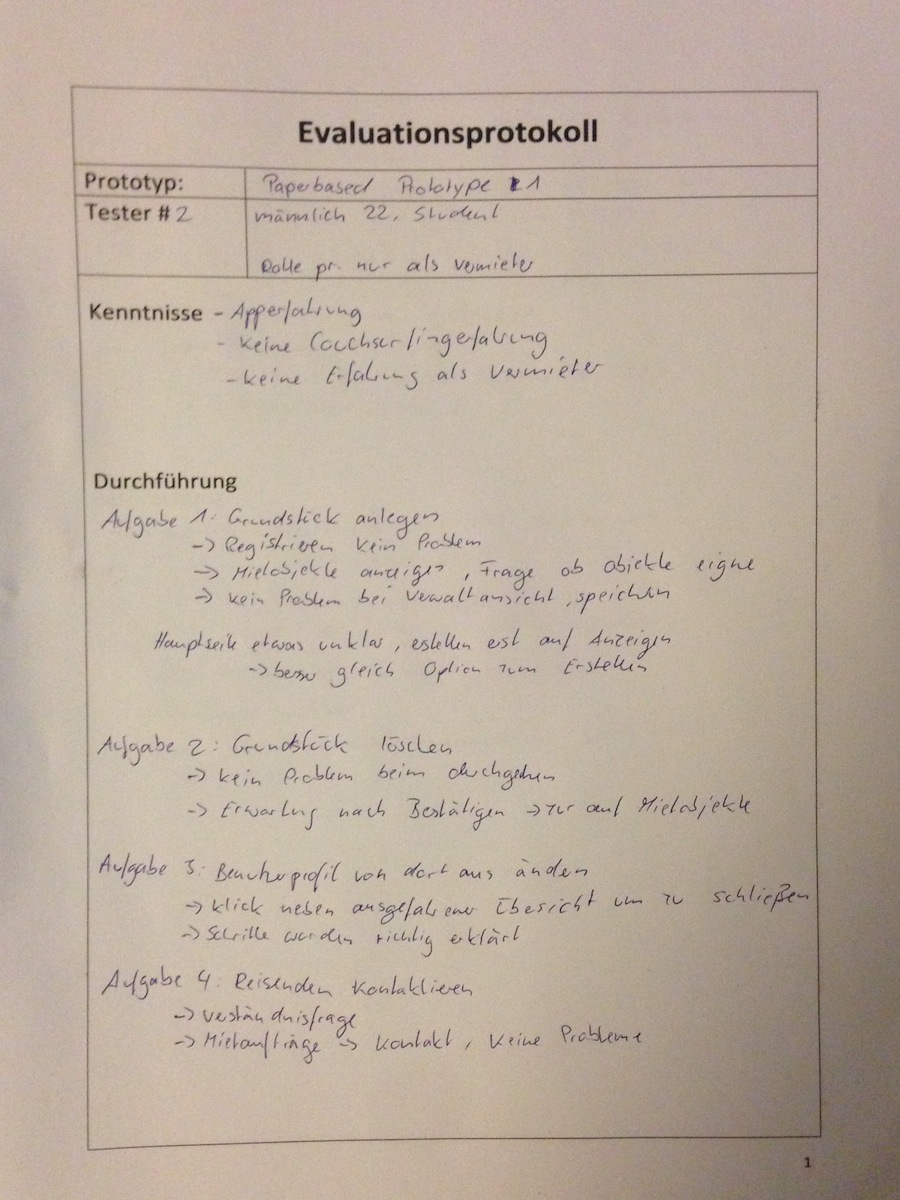
\includegraphics[width=1\textwidth]{./images/evaluation/eva21.JPG}
\caption{Evaluationsprotokoll 2.1}
\label{fig:evaluation21}
\end{figure}

Abb. \ref{fig:evaluation22}
\begin{figure}[H]
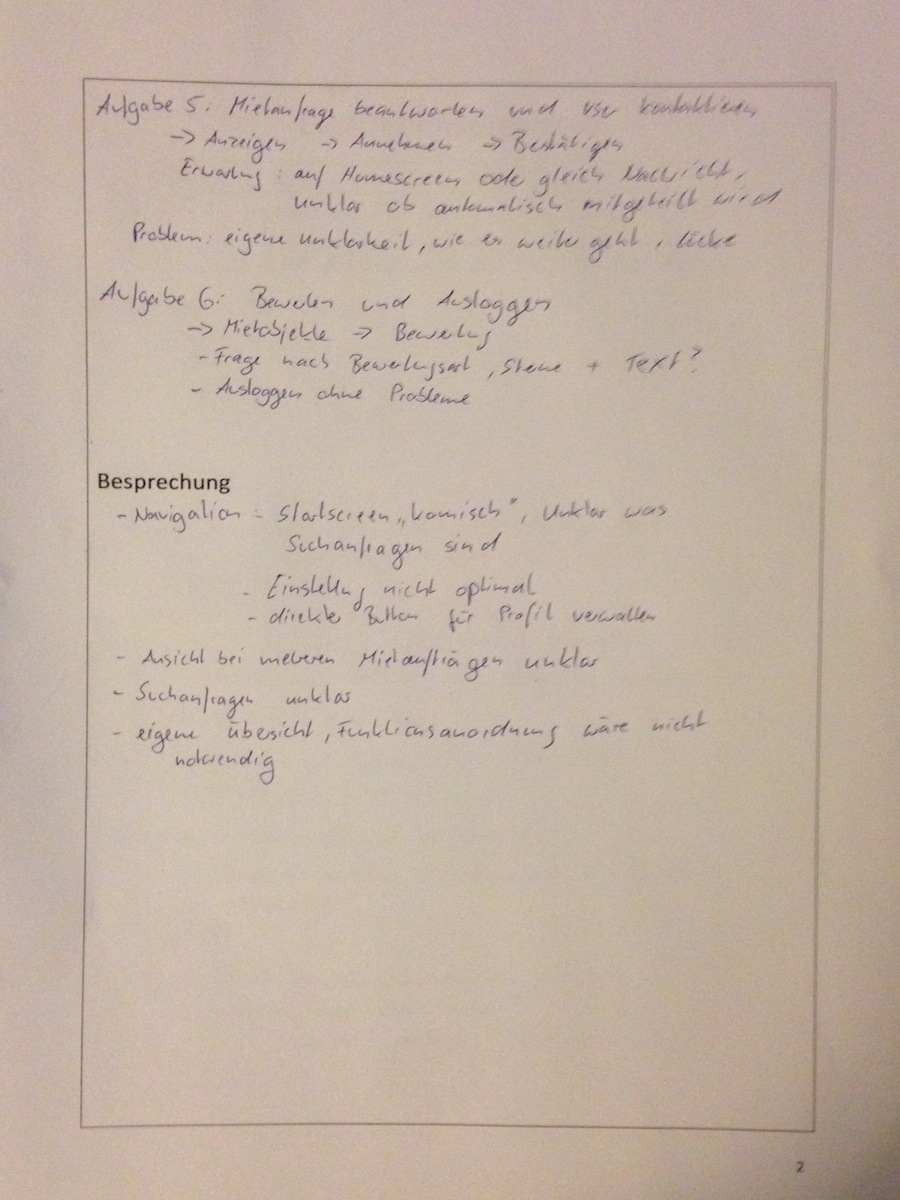
\includegraphics[width=1\textwidth]{./images/evaluation/eva22.JPG}
\caption{Evaluationsprotokoll 2.2}
\label{fig:evaluation22}
\end{figure}

Abb. \ref{fig:mainneu}
\begin{figure}[H]
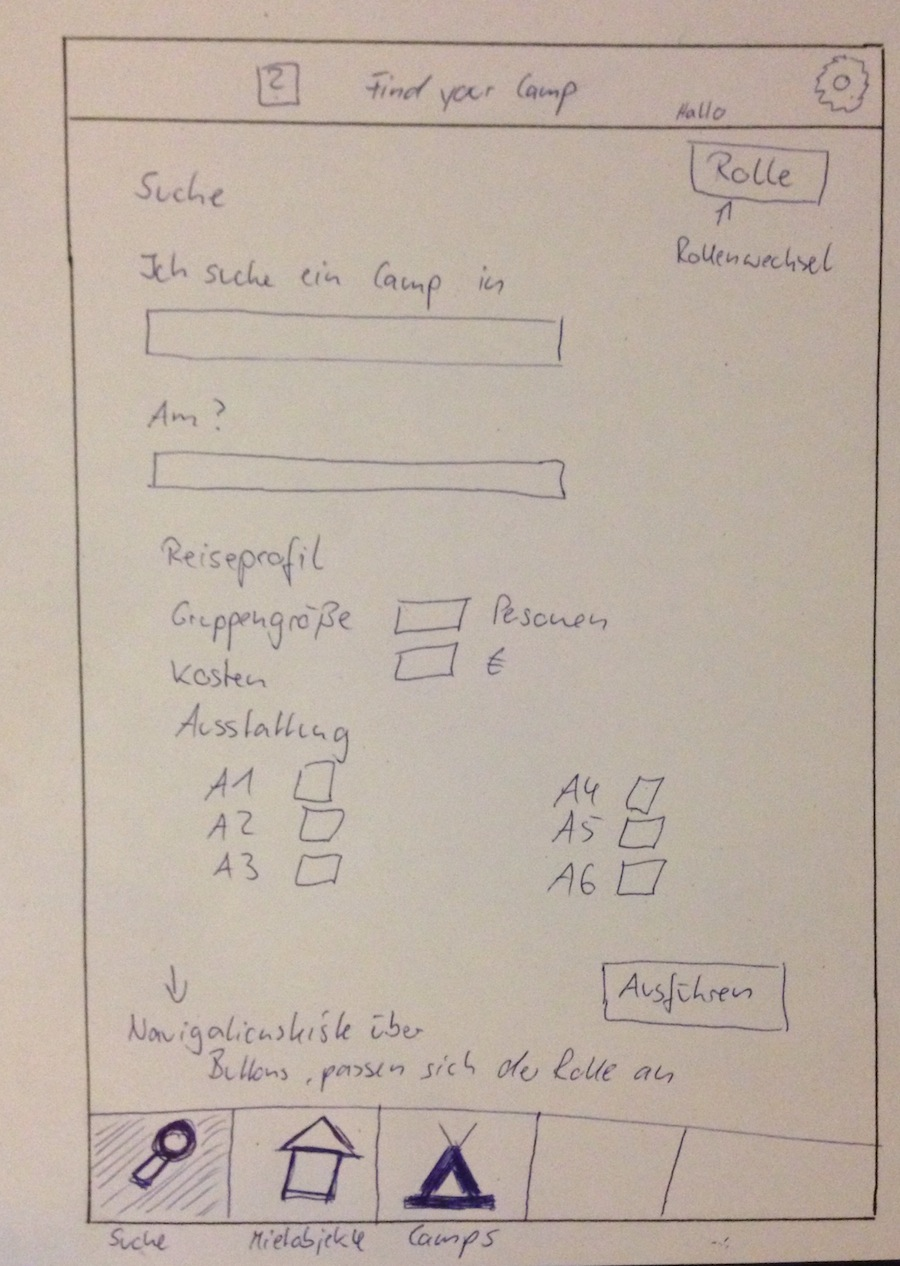
\includegraphics[width=1\textwidth]{./images/mainneu.JPG}
\caption{Evaluationsprotokoll 2.2}
\label{fig:mainneu}
\end{figure}

\subsection{Grundsätze der Dialoggestaltung}
 ISO 9241 Teil 110
 Gestaltungsempfehlungen ISO Teil 12-17
\\
 1. Aufgabenangemessenheit\\
 	Fokus auf Aufgabe, nicht auf Technik\\
 	Dialogsystem: nur Informationen für Aufgabe, Hilfefunktion, \\automatische Ausführung, Eingabe Cursor im ersten Eingabe Widget, bei wiederkehrenden Aufgaben unterstützen = Speichern von aufeinander folgenden Interaktionsschritten, Standartwerte als Vorgabewerte\\
\\
 2. Selbstbeschreibungsfähigkeit\\
    Verständnis zum aktuellen Standpunkt im Dialog, was gemacht werden kann, wie man es ausführt\\
    Rückmeldung durch unmittelbares Anzeigen der Eingaben, bei schwerwiegenden Folgen Bestätigung einbauen, keine Fachterminologie, Begriffe erläutern und Benutzerhandbuch, Informationen zum aktuellen Stand, zB prozentualer Beabreitungsstand, Überblick über zukünftige Dialogschritte, Informationen zum Eingabedatentyp

 3. Steuerbarkeit\\
 	Geschwindigkeit unter der Kontrolle des Benutzers, Dialogsystem setzt immer auf nächsten Eingabecursor, sollte aber freie Interaktion ermöglichen. Interaktionsschritte sollten zurücknehmbar sein, auch auf das zurückgreifen zuvor gelöschter Objekte, Short Cuts?

 4. Erwartungskonformität\\
 	konsistent, Merkmalen der Benutzern entsprechend, Zustandsmeldungen immer an der selben Stelle, Interaktionssequenz wird immer durch selbe Taste beendet, ähnlichkeiten, Antwortzeiten mitteilen, zB über ladebalken, status widget, prozentsatz des datenvolumens

 5. Fehlertoleranz\\
 	testen des Datentypens nach Eingabe, Fehler erläutern mit Fehlermeldung, farbige hervorhebung 

 6. Individualisierbarkeit\\
 	Anpassung an individuelle Fähigkeit und Bedürfnisse, Schriftgröße und Farbe, Sprache

 7. Lernförderlichkeit\\
 	Fehlerbeschreibung, learning by doing durch hohe Fehlertoleranz, Übungsszenarien\\

 	in weiteren Iso nachschauen
 	das Erkennen und Spezifizieren von Dialoganforderungen auf der Grundlage der verschiedenen Dialogtechniken, die in den Teilen der Norm ISO 9241-14 bis ISO 9241-17 beschrieben sind;
 den Entwurf von Gestaltungslösungen unter Einhaltung von ISO 9241-12 bis ISO 9241-17\\

 aus Benutzerperspektive gucken

 Gestaltungsanforderungen\\
 Gestaltungslösungen

 Nutzungskontext ist Quelle für DIaloganfordernungenTODO physische und soziale Arbeitsumgebung

 Gestaltung berücksichtigt gesamte User Experience\\
 Darstellung\\
 Funktionalität\\
 Systemleistung\\
 interaktiven Verhalten\\
 unterstützenden Ressourcen (Hardware und Software)\\
 + bisherigen Erfahrungen, Einstellungen, Fähigkeiten, Gewohnheiten und der Persönlichkeit des Benutzers\\

 organisatorische Auswirkungen, Benutzerdokumentation, Online-Hilfe, unterstützende Betreuung und Instandhaltung (einschliesslich Bera- tung und Kundenkontaktstellen), Schulung, langfristiger Gebrauch, und Produktverpackung (einschliesslich der Eindrücke bei der ers- ten Inbetriebnahme) sollten die Erfahrungen des Benutzers mit vor- herigen oder anderen Systemen und Probleme wie Markenkennzeich- nung und Werbung bedacht werden.\\

 Kontext sozialer kontext, alleine in der gruppe, ton an oder aus
 organisationaler kontext, zeit, ort

 Abstract Prototyping\\
 content of user interface ohne zu zeigen wie es aussieht\\

 Content Modeling \\
 inhalte des user interface ohne details zum aussehen
 content model = sammlung von material (was den user interessiert zu sehen oder zu ändern), tools (ermöglichen den user dies zu tun) und working spaces(teile die tools und materials verbinden)\\

 Papier = working spaces (post it = tools and materials)
 content model + navigation map

 conceptual scenarios£

\subsection{Sonstiges}

\subsubsection{Metaphern}
Icons können Metapher aktivieren und mentale Modelle erzeugen

